
\section{Protocolo Experimental}
	\label{sec:protocolo-experimental}



%%%%%%%%%% 
% Necessidade de uma referência
%%%%%%%%%%
Para que se possa avaliar um segmentador automático de textos, é preciso uma referência, isto é, um texto com os limites entre os segmento conhecidos. Essa referência, deve ser confiável, sendo uma segmentação legítima que é capaz de dividir o texto em porções relativamente independentes, mantendo um conteúdo legível, ou seja, uma segmentação ideal.
%

Entre as abordagens mais comuns para se conseguir essas referências, encontramos: A concatenação aleatória de documentos distintos, onde o ponto entre o final de um texto e o inicio do seguinte é um limite entre eles. A segmentação manual dos documentos, nesse caso, pessoas capacitadas, também chamadas de juízes, ou mesmo o autor do texto, são consultadas e indicam manualmente onde há uma quebra de segmento. Em transcrição de conversas faladas em reuniões com múltiplos participantes, um mediador é responsável por encerrar um assunto e iniciar um novo, nesse caso o mediador anota manualmente o tempo onde há uma transição de tópico. Em aplicações onde a segmentação é tarefa secundária, é possível, ao invés de avaliar o segmentador, analisar seu impacto na aplicação final.


%%%%%%%%%%
% As 2 principais dificuldades na avaliação
%%%%%%%%%%
De acordo com \cite{Pevzner2002} há duas principais dificuldades na avaliação de segmentadores automáticos. A primeira é conseguir um referência, já que juízes humanos costumam não concordar entre si, sobre onde os limites estão e outras abordagens podem não se aplicar ao contexto. A segunda é que tipos diferentes de erros devem ter pesos diferentes de acordo com a aplicação. Há casos onde certa imprecisão é tolerável e outras, como a segmentação de notícias, onde a precisão é mais importante.


%%%%%%%%%%
% Definição do que é um bom algoritmo de segmentação
%%%%%%%%%%
Para fins de avaliação desse trabalho, um bom método de segmentação é aquele cujo resultado melhor se aproxima do ideal, sem a obrigatoriedade de estar perfeitamente alinhado com tal. Ou seja, visto o contexto das atas de reunião, e a subjetividade da tarefa, não é necessário que os limites entre os segmentos (real e hipótese) sejam idênticos, mas que se assemelhem em localização e quantidade.


%Para quantificar a eficiência dos algoritmos, segue uma revisão das principais métricas aplicáveis.

As próximas subseções mostram o conjunto de atas e a segmentação usada como referência, uma revisão das principais métricas aplicáveis à segmentação e os testes realizados para avaliar os métodos.


\subsection{Conjunto de documentos}
	\label{subsec:conjunto-de-documentos}
	A fim de obter um conjunto de documentos segmentados que possam servir como referência na avaliação, seis atas de reunião foram coletadas junto ao departamento de pós-graduação da UFSCar-Sorocaba\footnote{\urlatas}. Os documentos foram oferecidos à profissionais que participam de reuniões desse departamento e por meio de um \textit{software} segmentaram o texto das atas conforme o julgamento de cada um. Os segmentos gerados manualmente foram comparados à segmentação automática conforme os critérios descritos a seguir.
	
	As atas de reunião diferem dos textos comumente estudados em outros trabalhos em alguns pontos. O estilo de escrita favorece textos sucintos com poucos detalhes de maneira que o ambiente dá preferência a textos curtos. Segundo Choi~\cite{Choi2001-LSA}, o segmentador tem a acurácia reduzida em segmentos curtos (em torno de 3 a 5 sentenças).
	
	Para evitar um texto monótono à leitura, a redação do documento tem o cuidado de não repetir ideias e palavras em favor da elegância do texto. Tal característica enfraquece a coesão léxica e portanto o cálculo da similaridade é prejudicado. Por exemplo, duas sentenças diferem se uma contiver a palavra \textit{computadores} e na seguinte \textit{equipamentos}, mesmo que se refiram à mesma ideia.
	
	Além disso, o documento compartilha um certo vocabulário próprio do ambiente onde os assuntos são discutidos e com isso nota-se que os segmentos, embora tratem de assuntos diferentes, são semelhantes em vocabulário.
	
A presença de ruídos como cabeçalhos, rodapés e numeração de páginas e linhas prejudicam tanto similaridade entre sentenças como a apresentação final ao usuário. Porém, esses ruídos podem ser reduzidos ou eliminados como mostrado na Subseção~\ref{subsec:preprocessamento}, sobre preprocessamento.


\subsection{Medidas de Avaliação}


	As medidas de avaliação tradicionalmente utilizadas em \textit{information retrieval} como precisão e revocação trazem alguns problemas na avalização de segmentadores automáticos.  
Conforme o algoritmo aponta mais segmentos no texto, tende a melhorar a revocação e ao mesmo tempo, reduzir a precisão, um problema que pode ser contornado usando \textit{F-measure} que faz uma combinação da duas levando em conta seus pesos, o que por outro lado é mais difícil de interpretar. 
Essas medidas falham ao não serem sensíveis a \textit{near misses}, ou seja, quando um limite não coincide exatamente com o esperado, mas fica próximo a ele~\cite{Kern2009}.

A Figura~\ref{fig:exemplosegmentacaozoom} mostra um exemplo com duas segmentações hipotéticas e uma referência. Na Figura~\ref{fig:exemplosegmentacao}, em ambos os casos não há nenhum verdadeiro positivo, o que implica em zero para os valores de precisão, acurácia, e revocação, embora a segunda hipótese possa ser considerada superior à primeira se levado em conta a proximidade dos limites.



  \begin{figure}[!h]

	\centering
	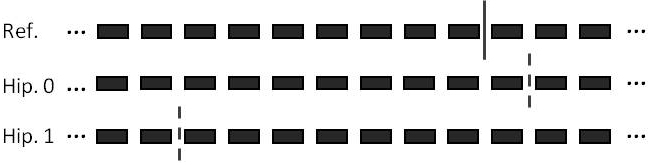
\includegraphics[width=0.47\textwidth]{windiffzoom.jpg}
	\caption{Exemplos de \textit{near missing} e falso positivo puro. Os blocos indicam uma unidade de informação e as linha verticais representam os limites entre segmentos. }
	\label{fig:exemplosegmentacaozoom}

  \end{figure}
  
  \begin{figure}[!h]

	\centering
	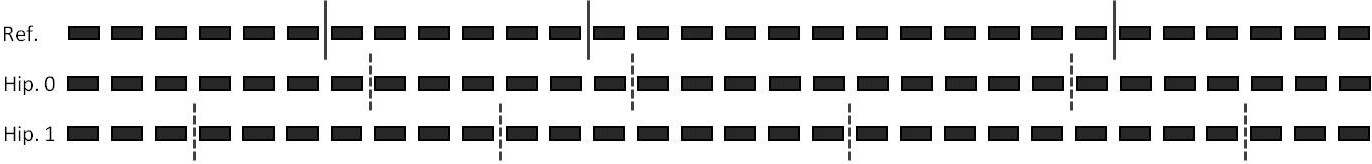
\includegraphics[width=0.47\textwidth]{windiff.jpg}
	\caption{
	Exemplo de duas segmentações hipotéticas em comparação a uma ideal. 
	}
	\label{fig:exemplosegmentacao}

  \end{figure}
  
  
Entre as medidas mais utilizadas para avaliar segmentadores estão:

\subsubsection{P$_k$}
A fim de resolver o problema de \textit{near misses}, Beeferman \textit{et. al.}~\cite{Beeferman1999} apresentam uma nova medida chamada P$_k$ que atribui valores parciais a \textit{near misses}. Esse método move uma janela de tamanho $k$ e a cada posição e verifica se o início e o final da janela estão ou não dentro do mesmo segmento e penaliza o algoritmo em caso de discrepância. 

Ou seja, dado duas palavras de distancia $k$, uma discrepância é computada quando o algoritmo e a referência não concordam se as palavras estão ou não no mesmo segmento.

O valor de $k$ é calculado como a metade da média dos comprimentos dos segmentos reais. Como resultado, é retornado a contagem de discrepâncias divido pelo quantidade de segmentações analisadas. Esse valor serve como medida de dissimilaridade entre as segmentações e pode ser interpretada como a probabilidade de duas sentenças extraídas aleatoriamente pertencerem ao mesmo segmento.



\subsubsection{WindowDiff}

Pevzner~\cite{Pevzner2002} aponta problemas na avaliação mais tradicional P$_k$~\cite{Beeferman1999}. Eles apontam que esse método penaliza demasiadamente os falsos negativos em relação aos falsos positivos e a \textit{near misses}, além disso, desconsidera o tamanho e a quantidade de segmentos, entre outros problemas.

Como solução, propõem um novo método, o qual chamam de \textit{WindowDiff} que traz duas diferenças principais: a dobra a penalidade para os falsos positivos a fim de diminuir o problema da subestimação dessa medida e, diferente de P$_k$, ao mover a janela pelo texto, penaliza o algoritmo sempre que o número de limites proposto pelo algoritmo não coincidir com o número de limites esperados para aquela janela de texto. 

Com isso, demonstram em seu trabalho que, em relação a P$_k$, consegue resolver seus principais problemas e mantém sua proposta inicial de sensibilidade a \textit{near misses}, penalizando-os menos que os falsos positivos puros.


  

%Falar do software para segmentação manual????






